\begin{itemize}
    \item Location of a point on a line
    \begin{quote}
        \textit{
            Imagine a world where you can only move in two directions: forward and backward. You can't move left or right, up or down—only along a single straight path. This path is called the x-axis. The x-axis is a horizontal line that extends infinitely in both directions. \\[2mm]
            In this one-dimensional world, we can describe the location of any point using a single number, which we call the coordinate of that point. This number tells us exactly how far along the x-axis the point is from a specific reference point known as the origin. The origin is the center point of the x-axis and has a coordinate of $0$.\\[2mm]
            If a point has a positive coordinate, it means the point is to the right of the origin. If a point has a negative coordinate, it means the point is to the left of the origin. The greater the number, the further the point is from the origin.
        }
    \end{quote}

        \begin{center}
            \begin{tikzpicture}
                \tzaxes(-5, 0)(5, 0.15){$x$}{}
                \tzticks{-4/$-4$, -3/$-3$, -2/$-2$, -1/$-1$, 0/$0$, 1/$1$, 2/$2$, 3/$3$, 4/$4$}{}
                \tzticks*{-4, -3, -2, -1, 1, 2, 3, 4}{}
            \end{tikzpicture}
            \begin{tikzpicture}
                \tzaxes(-5, 0)(5, 0.15){$x$}{}
                \tzticks{-2.5/$x_1$, 2.5/$x_2$}{}
                \tzticks*{-2.5, 0, 2.5}{}
                \tzline[|<->|]<0, -0.75>(-2.5, 0)(2.5, 0){$x_2 - x_1$}[mb]
            \end{tikzpicture}
        \end{center}

    \item Location of a point in a plane
    \begin{quote}
        \textit{
            Now, imagine a world where you can move not just forward and backward, but also left and right. This world is two-dimensional, meaning it has two directions or axes along which you can move: the x-axis and the y-axis.\\[2mm]
            The x-axis is a horizontal line that runs from left to right, and the y-axis is a vertical line that runs from bottom to top. These two lines intersect at a point called the origin, which has the coordinates (0, 0).
            In this two-dimensional world, we can describe the location of any point using a pair of numbers called coordinates. These coordinates are written as (x, y):\\[2mm]
            The first number, x, tells us how far along the x-axis the point is from the origin. A positive x value means the point is to the right of the origin, while a negative x value means the point is to the left.
            The second number, y, tells us how far along the y-axis the point is from the origin. A positive y value means the point is above the origin, while a negative y value means the point is below.
        }
    \end{quote}

        \begin{center}
            \begin{tikzpicture}
                \tzaxes(-5, -3)(5, 4){$x$}{$y$}
                \tzticks*{-4, -3, -2, -1, 1, 2, 3, 4}{-2, -1, 1, 2, 3}
                \tzcoor*(0, 0)(O){$O$}[bl]
                \tzcoor*(2, 3)(P){$P(2,3)$}[ar]
                \tzline[|<->|]<0, -0.5>(0, 0)(2, 0){$2$}[mb]
                \tzline[|<->|]<2.5, 0>(0, 0)(0, 3){$3$}[mr]
            \end{tikzpicture}
        \end{center}

        \textbf{Coordinates of a point $P(x, y)$:} \\
        
        \begin{itemize}
            \item \textbf{Distance between two points:}
                \begin{center}
                    \begin{tikzpicture}
                        \tzaxes(-2, -1.5)(7, 4){$x$}{$y$}
                        \tzcoor*(0, 0)(O){$O$}[bl]
                        \tzcoor*(2, 3)(P){$P(x_1, y_1)$}[ar]
                        \tzcoor*(5, 1)(Q){$Q(x_2, y_2)$}[ar]
                        \tzline[dashed](2, 1)(5, 1){$x_2-x_1$}[mb]
                        \tzline[dashed](2, 1)(2, 3){$y_1-y_2$}[ml]
                        \tzline(P)(Q){$d$}[ma]
                        \tzline[|<->|]<0, -0.5>(0, 0)(2, 0){$x_1$}[mb]
                        \tzline[|<->|]<0, -1>(0, 0)(5, 0){$x_2$}[mb]
                        \tzline[|<->|]<-0.5, 0>(0, 0)(0, 1){$y_2$}[ml]
                        \tzline[|<->|]<-1, 0>(0, 0)(0, 3){$y_1$}[ml]
                    \end{tikzpicture}
                \end{center}
                \begin{align*}
                    \intertext{Distance between two points $P(x_1, y_1)$ and $Q(x_2, y_2)$:}
                    \intertext{Using Pythagoras theorem:}
                    \Aboxed{d &= \sqrt{(x_2 - x_1)^2 + (y_2 - y_1)^2}}
                \end{align*}

            \item \textbf{Midpoint of a line segment:}
                \begin{center}
                    \begin{tikzpicture}
                        \tzcoor*(2, 3)(P){$P(x_1, y_1)$}[ar]
                        \tzcoor*(5, 1)(Q){$Q(x_2, y_2)$}[ar]
                        \tzcoor*(3.5, 2)(M){$M(x_m, y_m)$}[ar]
                        \tzline[dashed](2, 1)(5, 1){$x_2-x_1$}[mb]
                        \tzline[dashed](2, 1)(2, 3){$y_1-y_2$}[ml]
                        \tzline(P)(Q)
                        \tzline[dashed](2, 2)(M){$x_m-x_1$}[mb]
                        \tzline[dashed, |<->|]<-1.5, 0>(2, 2)(2, 3){$y_1-y_m$}[ml]
                    \end{tikzpicture}
                \end{center}
                \begin{align*}
                    \intertext{Midpoint of a line segment $P(x_1, y_1)$ and $Q(x_2, y_2)$:}
                    \intertext{From the above diagram, we can see that both the triangles are similar.}
                    \intertext{Therefore,}
                    \frac{y_1-y_m}{y_1-y_2} &= \frac{x_m-x_1}{x_2-x_1} = \frac{PM}{PQ} \\
                    \intertext{As the midpoint divides the line segment into two equal parts,}
                    \frac{y_1-y_m}{y_1-y_2} &= \frac{x_m-x_1}{x_2-x_1} = \frac{1}{2}
                \end{align*}
                \begin{align*}
                    \intertext{Solve for $x_m$ and $y_m$:}
                    \frac{x_m - x_1}{x_2 - x_1} &= \frac{1}{2}  &\text{and}&& \frac{y_1 - y_m}{y_1 - y_2} &= \frac{1}{2} \\
                    x_m - x_1 &= \frac{x_2 - x_1}{2}  &\text{and}&& y_1 - y_m &= \frac{y_1 - y_2}{2} \\
                    x_m &= \frac{x_1 + x_2}{2}  &\text{and}&&  y_m &= \frac{y_1 + y_2}{2}
                \end{align*}
                \begin{align*}
                    \Aboxed{M(x_m, y_m) &= \left(\frac{x_1 + x_2}{2}, \frac{y_1 + y_2}{2}\right)}
                \end{align*}
        \end{itemize}

\end{itemize}
